%!TEX root = ../dissertation.tex


\chapter{Deterministic}
\label{deterministic}


%!TEX root = ../dissertation.tex


\chapter{Data}
\label{data}


%!TEX root = ../dissertation.tex


\section{Deterministic Results}
\label{dresults}


\subsection{25.4 mm Threshold}
\label{dresults_25.4mm}

It is readily apparent from \mbox{Figure \ref{single_25comp}} that the centroid of the two-dimensional frequency distribution is observed to the north-northeast of the representative forecast grid point and the distribution has an elliptical shape.
When the anisotropic Gaussian function is fit to this distribution, the resulting parameters, determined by the methods discussed in \mbox{chapter \ref{method}} and \cite{Lak2010}, are $(\mu_x, \mu_y) = (4.7, 18.8)$ kilometers, indicating that the NSSL-WRF forecasts were, on average, approximately \mbox{4.7 km} too far west and \mbox{18.8 km} too far south, $\sigma_x \approx 190$ kilometers, $\sigma_y \approx 155$ kilometers, and $\theta \approx 60^{\circ}$ in the counter-clockwise direction, revealing the anisotropy of the distribution.
To some extent, the shape and anisotropy are closely related to the mean shape and orientation of individual precipitation objects, as revealed by comparing the average size-weighted orientation of the precipitation objects, determined by the Baldwin object identification algorithm \citep{Baldwin2005}, to the orientation angle of the fitted distribution (not shown).


Using this fitted two-dimensional distribution, probabilistic forecasts for each \mbox{6-hr} time period from 01 April 2010 --- 31 March 2011 were generated in a manner similar to what was done by \cite{Sobash2011}, except that the shifted, fitted distribution was used instead of the simple isotropic Gaussian.
Four sample forecasts, all of differing lead times, are shown in \mbox{Figures \ref{single_1_400km_25mm}} and \ref{single_2_400km_25mm} and are now discussed.
However, one must be cautious about assessing the skill of a probabilistic forecasting system on the basis of individual events.


\mbox{Figures \ref{single_1_400km_25mm}a}, \mbox{\ref{single_1_400km_25mm}c}, and \mbox{\ref{single_1_400km_25mm}e} depict observations and model forecasts of precipitation for the 6-hrs ending 18 UTC 2 May 2010 (a 12-18 hr forecast).
During this 6-hr period, heavy-rain fell over an elongated area stretching from central Mississippi north-northeastward into southeastern Ohio and western West Virginia, with an area exceeding 200 mm in north-central Tennessee \mbox{(Figure \ref{single_1_400km_25mm}a)}.
South and east of this axis of heaviest rainfall, areas in eastern Mississippi had precipitation totals around the 25.4 mm threshold.
The NSSL-WRF forecast of this event was generally good, cluing forecasters in on the general area of concern.
However, the NSSL-WRF forecast had three distinct areas of heavy rain compared to the single large band that was observed: one northwest of the observed axis of heavy rain, one southeast, and one along the northeastern most observed area exceeding 25.4 mm \mbox{(Figure \ref{single_1_400km_25mm}c)}.
Applying the proposed probabilistic method resulted in the area of highest probabilities of reaching or exceeding 25.4 mm (between 25 and 30\%) occurring very near the area of maximum rainfall \mbox{(Figure \ref{single_1_400km_25mm}e)}.
Additionally, the axis of highest probabilities extending northeast of the maximum probabilities aligned very well with the observed area equal to or exceeding 25.4 mm.
The axis of highest probabilities also extends to the south and southwest of the maximum forecast probabilities, capturing the southwestward extent of the observed heavy rain, at the same time highlighting areas in eastern Mississippi \mbox{(Figure \ref{single_1_400km_25mm}e)}.


\mbox{Figsures \ref{single_1_400km_25mm}b}, \mbox{\ref{single_1_400km_25mm}d}, and \mbox{\ref{single_1_400km_25mm}f} depict observations and model forecasts of precipitation for the 6-hrs ending 00 UTC 27 September 2010 (an 18-24 hr forecast).
Observations depict a large area of precipitation greater than or equal to 25.4 mm stretching from southeastern Alabama northeastward into far northwestern South Carolina with scattered areas reaching this threshold across southern Mississippi and eastern North and South Carolina \mbox{(Figure \ref{single_1_400km_25mm}b)}.
The NSSL-WRF forecast of this event depicted two areas exceeding 25.4 mm of precipitation, essentially capturing both observed areas (\mbox{cf. Figures \ref{single_1_400km_25mm}b} and \mbox{\ref{single_1_400km_25mm}d)}.
The corridor of observations greater than 25.4 mm are generally contained within 5-10\% probabilities \mbox{(Figure \ref{single_1_400km_25mm}f)}. In this case, much of the area covered by the highest probabilities of 15-20\% did not receive heavy rainfall during this period.


A 24-30 hr forecast and observations of precipitation for the 6-hrs ending 06 UTC 06 June 2010 are presented in \mbox{Figures \ref{single_2_400km_25mm}a}, \mbox{\ref{single_2_400km_25mm}c}, and \mbox{\ref{single_2_400km_25mm}e}.
Observations depict two areas over Michigan that reach the 25.4 mm threshold.
The first extends from the southeastern portion of Lake Michigan eastward to the western portions of Lake Erie.
The second area extends from the northern portion of Lake Michigan eastward to the western portions of Lake Huron.
A third area reaching the 25.4 mm threshold is found across Illinois and into Indiana \mbox{(Figure \ref{single_2_400km_25mm}a)}.
Although slightly farther west, the NSSL-WRF deterministic forecast does a reasonable job depicting the general location of the heaviest precipitation across Illinois and southern Michigan.
However, it under-predicts the heavy precipitation across northern Michigan \mbox{(Figure \ref{single_2_400km_25mm}c)}.
The probabilistic forecast derived from the NSSL-WRF captures most, if not all, observed areas that reached the 25.4 mm threshold with a probability of at least 5\% -- including the area across northern Michigan that was not explicitly forecast to exceed 25.4 mm by the deterministic forecast.
Furthermore, the highest probabilities are located in southwestern Michigan (30-35\%), conjoined with the western portion of the southern Michigan heavy rain axis \mbox{(Figure \ref{single_2_400km_25mm}e)}.


A 30-36 hr forecast and observations of precipitation for the 6-hrs ending 12 UTC 30 September 2010 are presented in \mbox{Figures \ref{single_2_400km_25mm}b}, \mbox{\ref{single_2_400km_25mm}d}, and \mbox{\ref{single_2_400km_25mm}f}.
Observations depict a large area exceeding the 25.4 mm threshold extending from eastern South Carolina, northward into far southeastern New York (Figure \mbox{\ref{single_2_400km_25mm}b)}.
Additionally, a small region of precipitation reaching the 25.4 mm threshold is found across northeastern Georgia.
The NSSL-WRF deterministic forecast is slightly narrower and farther east with its forecast, misplacing the axis of heaviest precipitation across North Carolina and Virginia \mbox{(Figure \ref{single_2_400km_25mm}d)}.
However, the NSSL-WRF generated probabilities encompass the area exceeding the 25.4 mm threshold, with the maximum probabilities of 40-45\% near Washington D.C. \mbox{(Figure \ref{single_2_400km_25mm}f)}.
The NSSL-WRF deterministic forecast completely missed the heavy precipitation across northeastern Georgia, and this area is sufficiently far from the area to the east that it falls outside the 0.1\% contour of the probabilistic forecast.


These examples are illuminating but many events are required to assess the skill of probabilistic forecast systems.
A more objective verification is provided here by applying well-known verification metrics to the entire 12-months worth of forecasts generated in this manner.
First, a Relative Operating Characteristic curve \citep{Mason1982} is computed from all forecasts and observations \mbox{(Figure \ref{single_verif_400km_25mm}a)}.
The resulting curve yields an area under the curve (AUC) of 0.94, indicating that the probabilistic forecasts have considerable skill in discriminating between events and non-events.
In order to visualize the reliability of the generated probabilistic forecasts, a reliability diagram was constructed (Figure \mbox{\ref{single_verif_400km_25mm}b)}.
The resulting diagram indicates that forecasts are quite reliable over a broad range of probabilities.




\subsection{12.7 mm Threshold}
\label{dresults_12.7mm}





As is apparent, this technique offers a method of objectively generating calibrated probabilistic forecasts of RCEs from a single deterministic model.
This technique is successful because it objectively represents, and corrects for, the mean displacement (systematic error) and the spatial uncertainty associated with the underlying deterministic forecast system (random error).
Preliminary assessments suggest that this uncertainty varies systematically as a function of numerous factors, such as forecast lead time, geographic location, meteorological season and regime, etc.
Further refinements to the technique could include dependencies on these factors.
For example, since cool-season precipitation forecasts tend to be more accurate than those for the warm-season, Gaussian fits to the position-error fields could vary as a function of season, with sharper, higher amplitude distributions in the cool-season and broader, lower amplitude distributions in the warm-season.








% CHAPTER FIGURES HERE --- Ensures they all show up at end of chapter

\clearpage
\begin{figure}[cc]
    \centering
    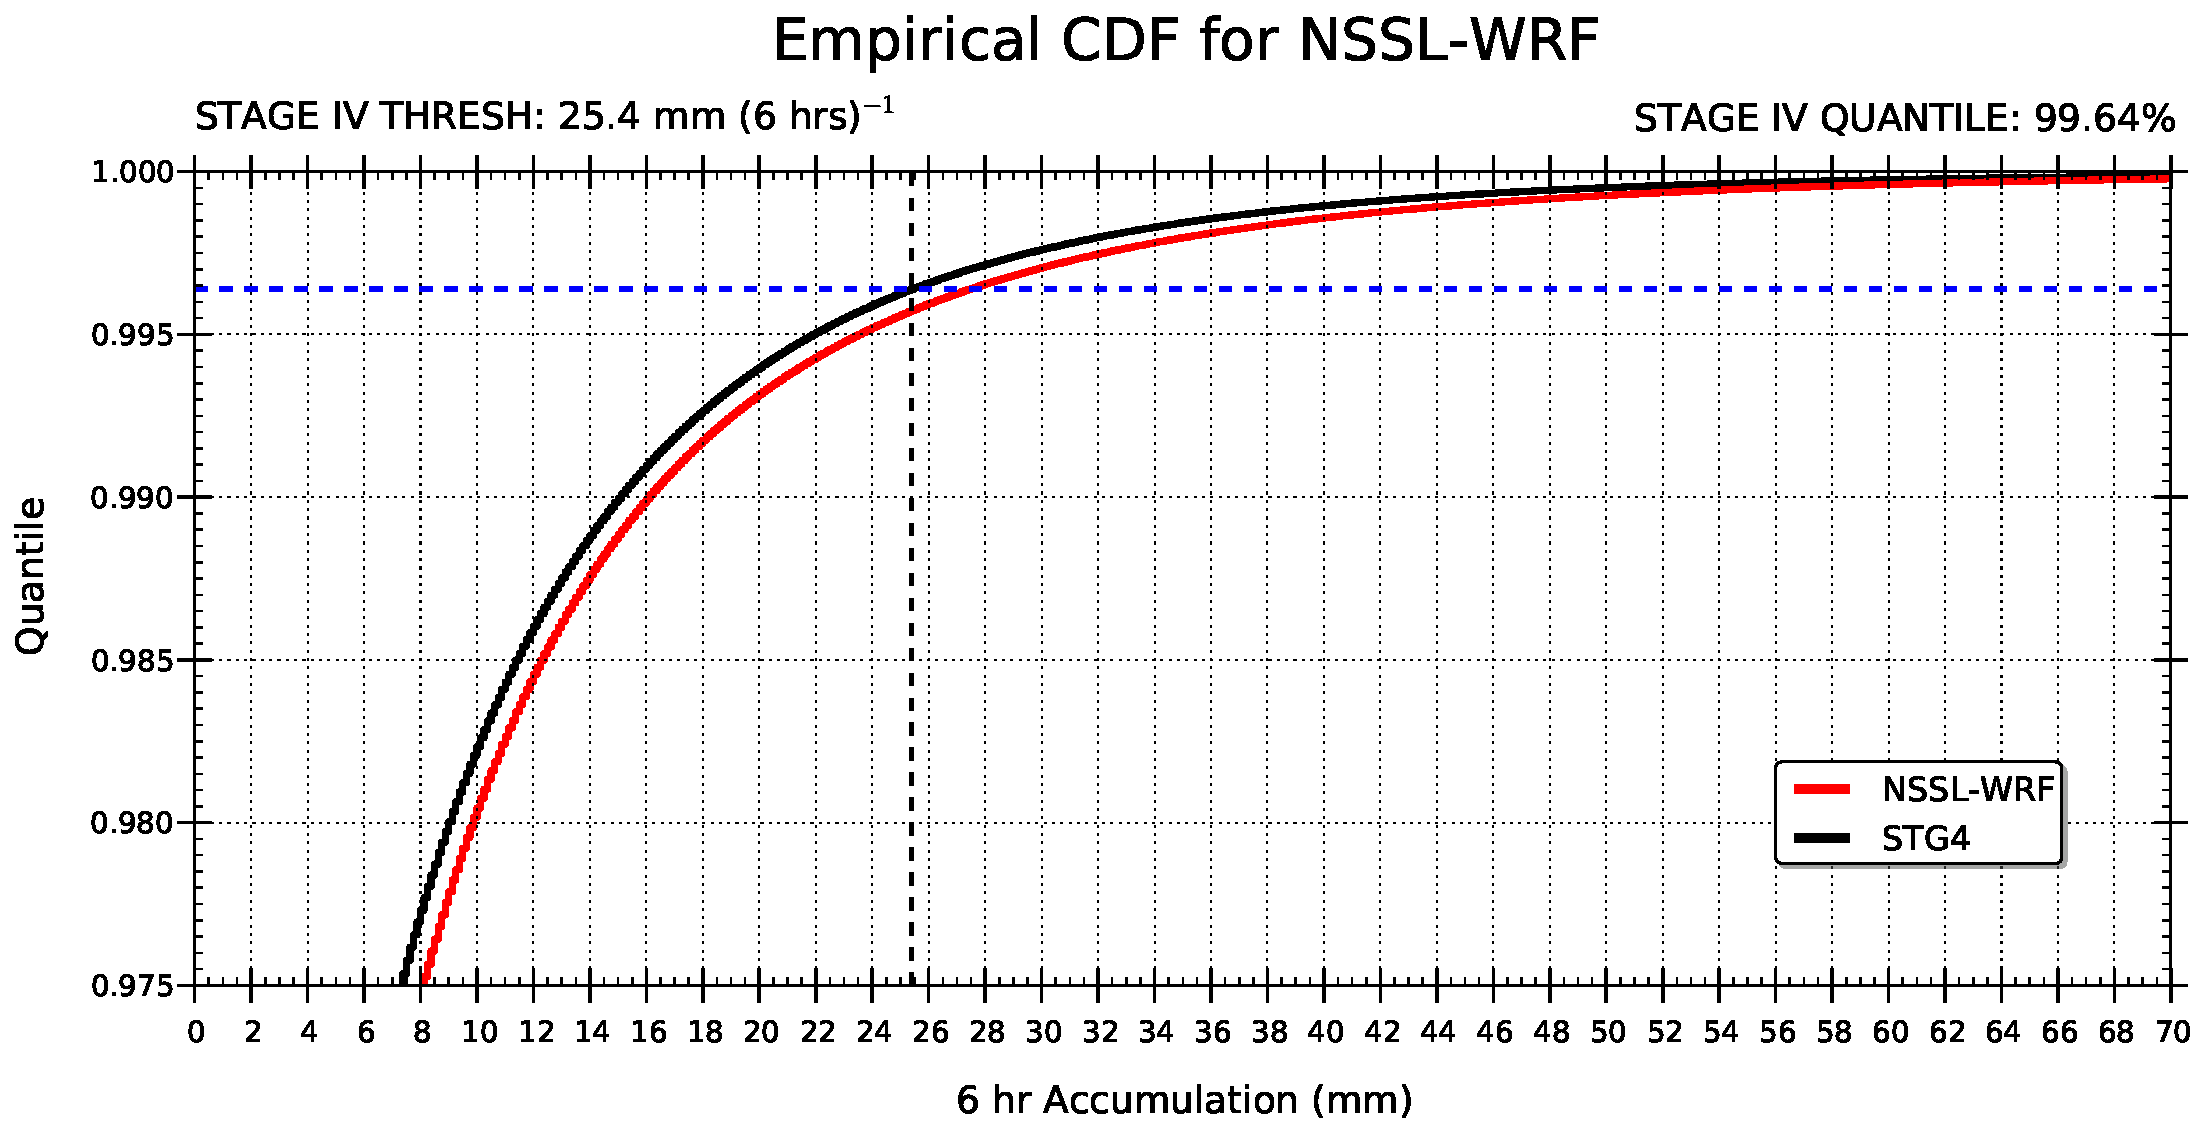
\includegraphics[width=\textwidth, height=\textheight, keepaspectratio]{%
    ./deterministic/figs/ecdf-nsslwrf-25mm}\\
    \caption{The empirical cumulative distribution function for both the Stage IV observations (black) and the NSSL-WRF forecasts (red), derived over the time period 01 April 2007 -- 31 March 2010.
    The vertical black dashed line is the \mbox{25.4 mm} threshold.
    The horizontal blue dashed line is the Stage IV quantile associated with the \mbox{25.4 mm} threshold.
    The NSSL-WRF distribution reaches this quantile at the \mbox{27.625 mm} threshold, as indicated by the horizontal blue dashed line.}
    \label{single_25quant}
\end{figure}


\clearpage
\begin{figure}[cc]
    \centering
    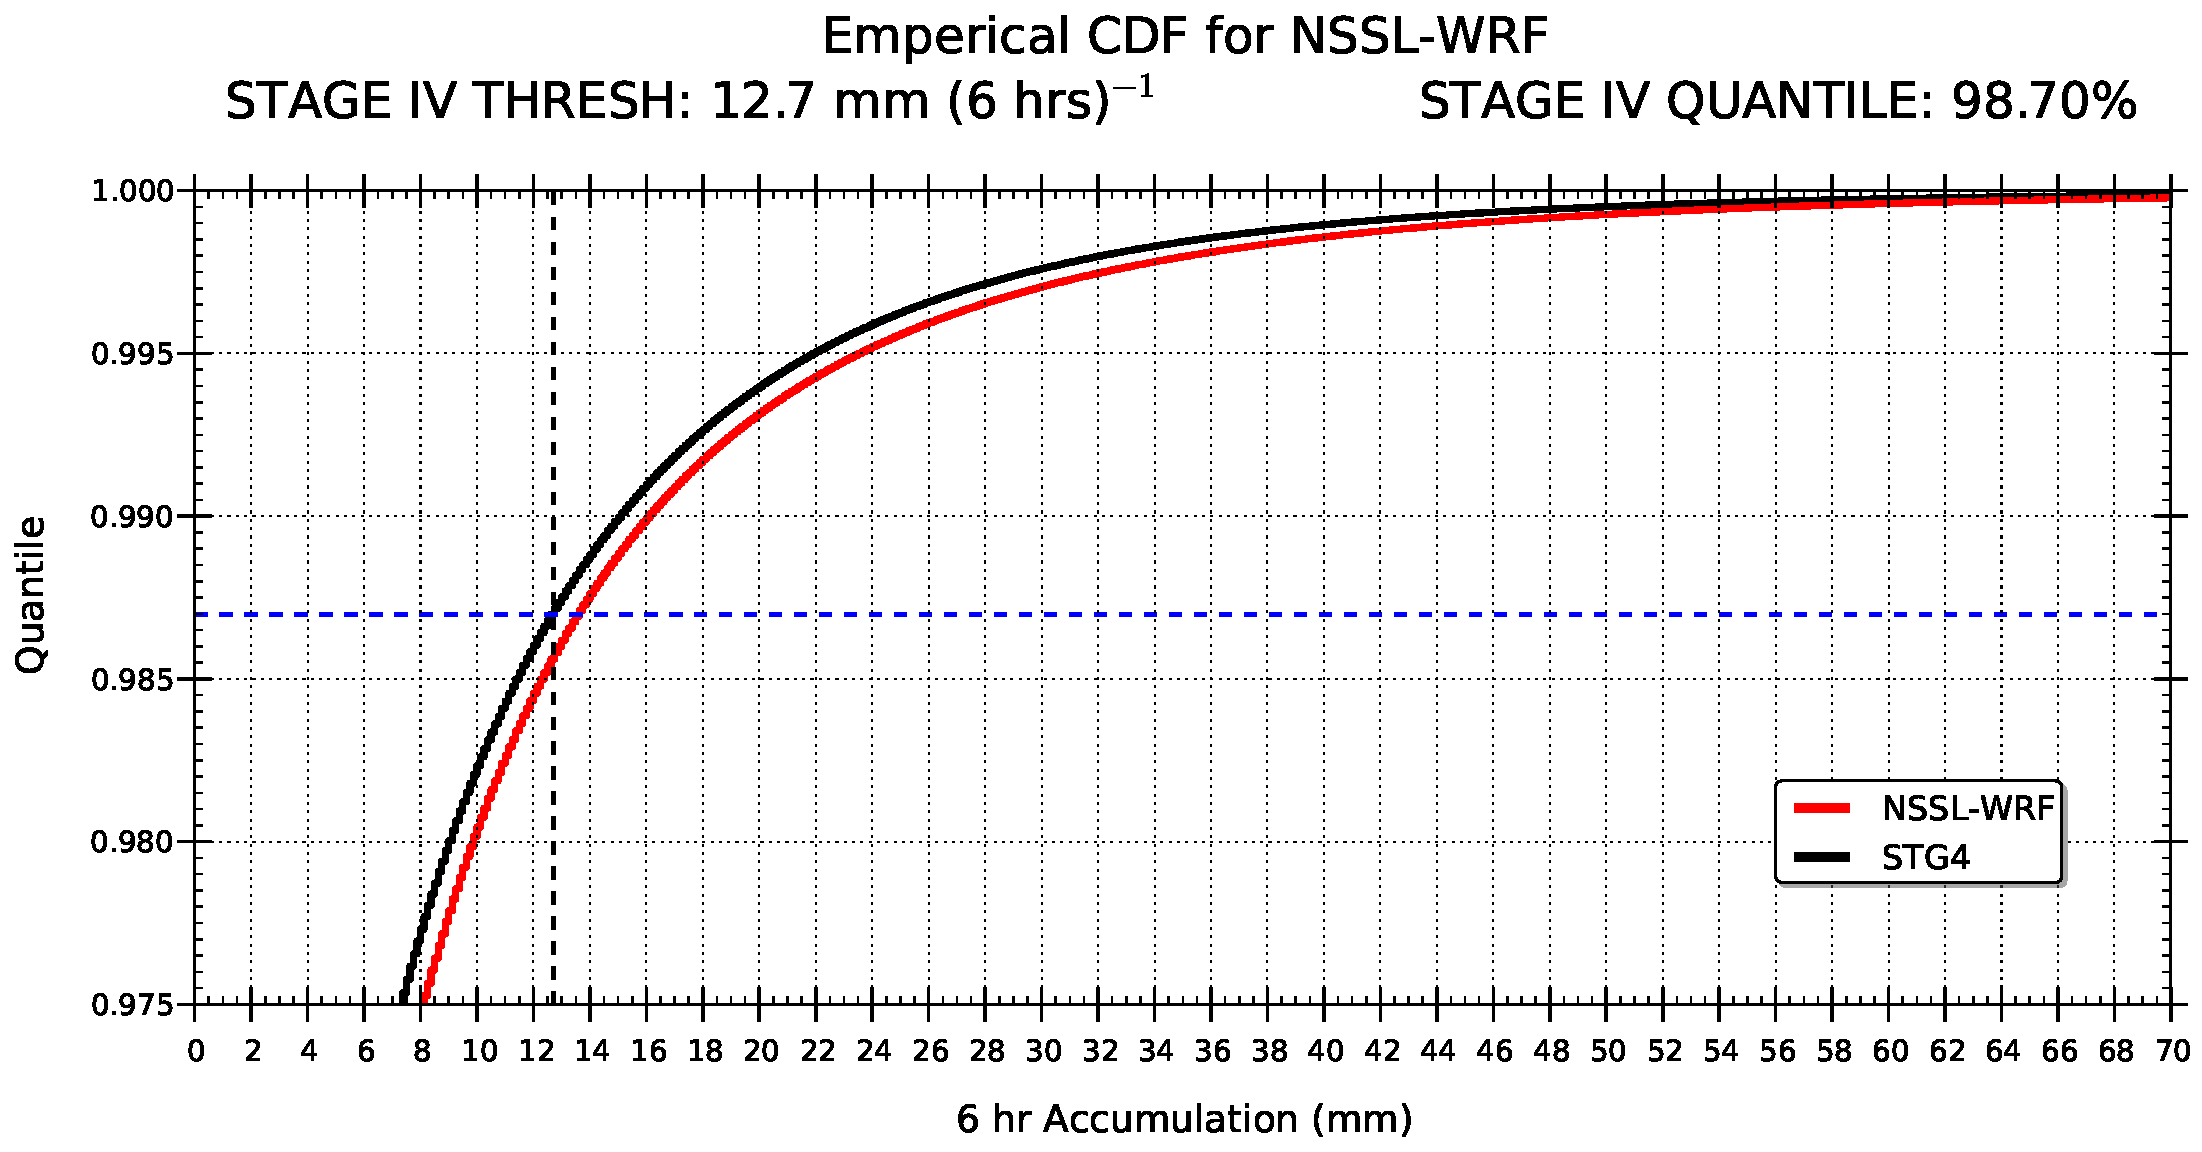
\includegraphics[width=\textwidth, height=\textheight, keepaspectratio]{%
    ./deterministic/figs/ecdf-nsslwrf-12mm}\\
    \caption{The same as in \mbox{Figure \ref{single_25quant}}, but using the \mbox{12.7 mm} threshold.
    The new threshold for the NSSL-WRF is \mbox{13.75 mm}.}
    \label{single_12quant}
\end{figure}


\clearpage
\begin{figure}[cc]
    \centering
    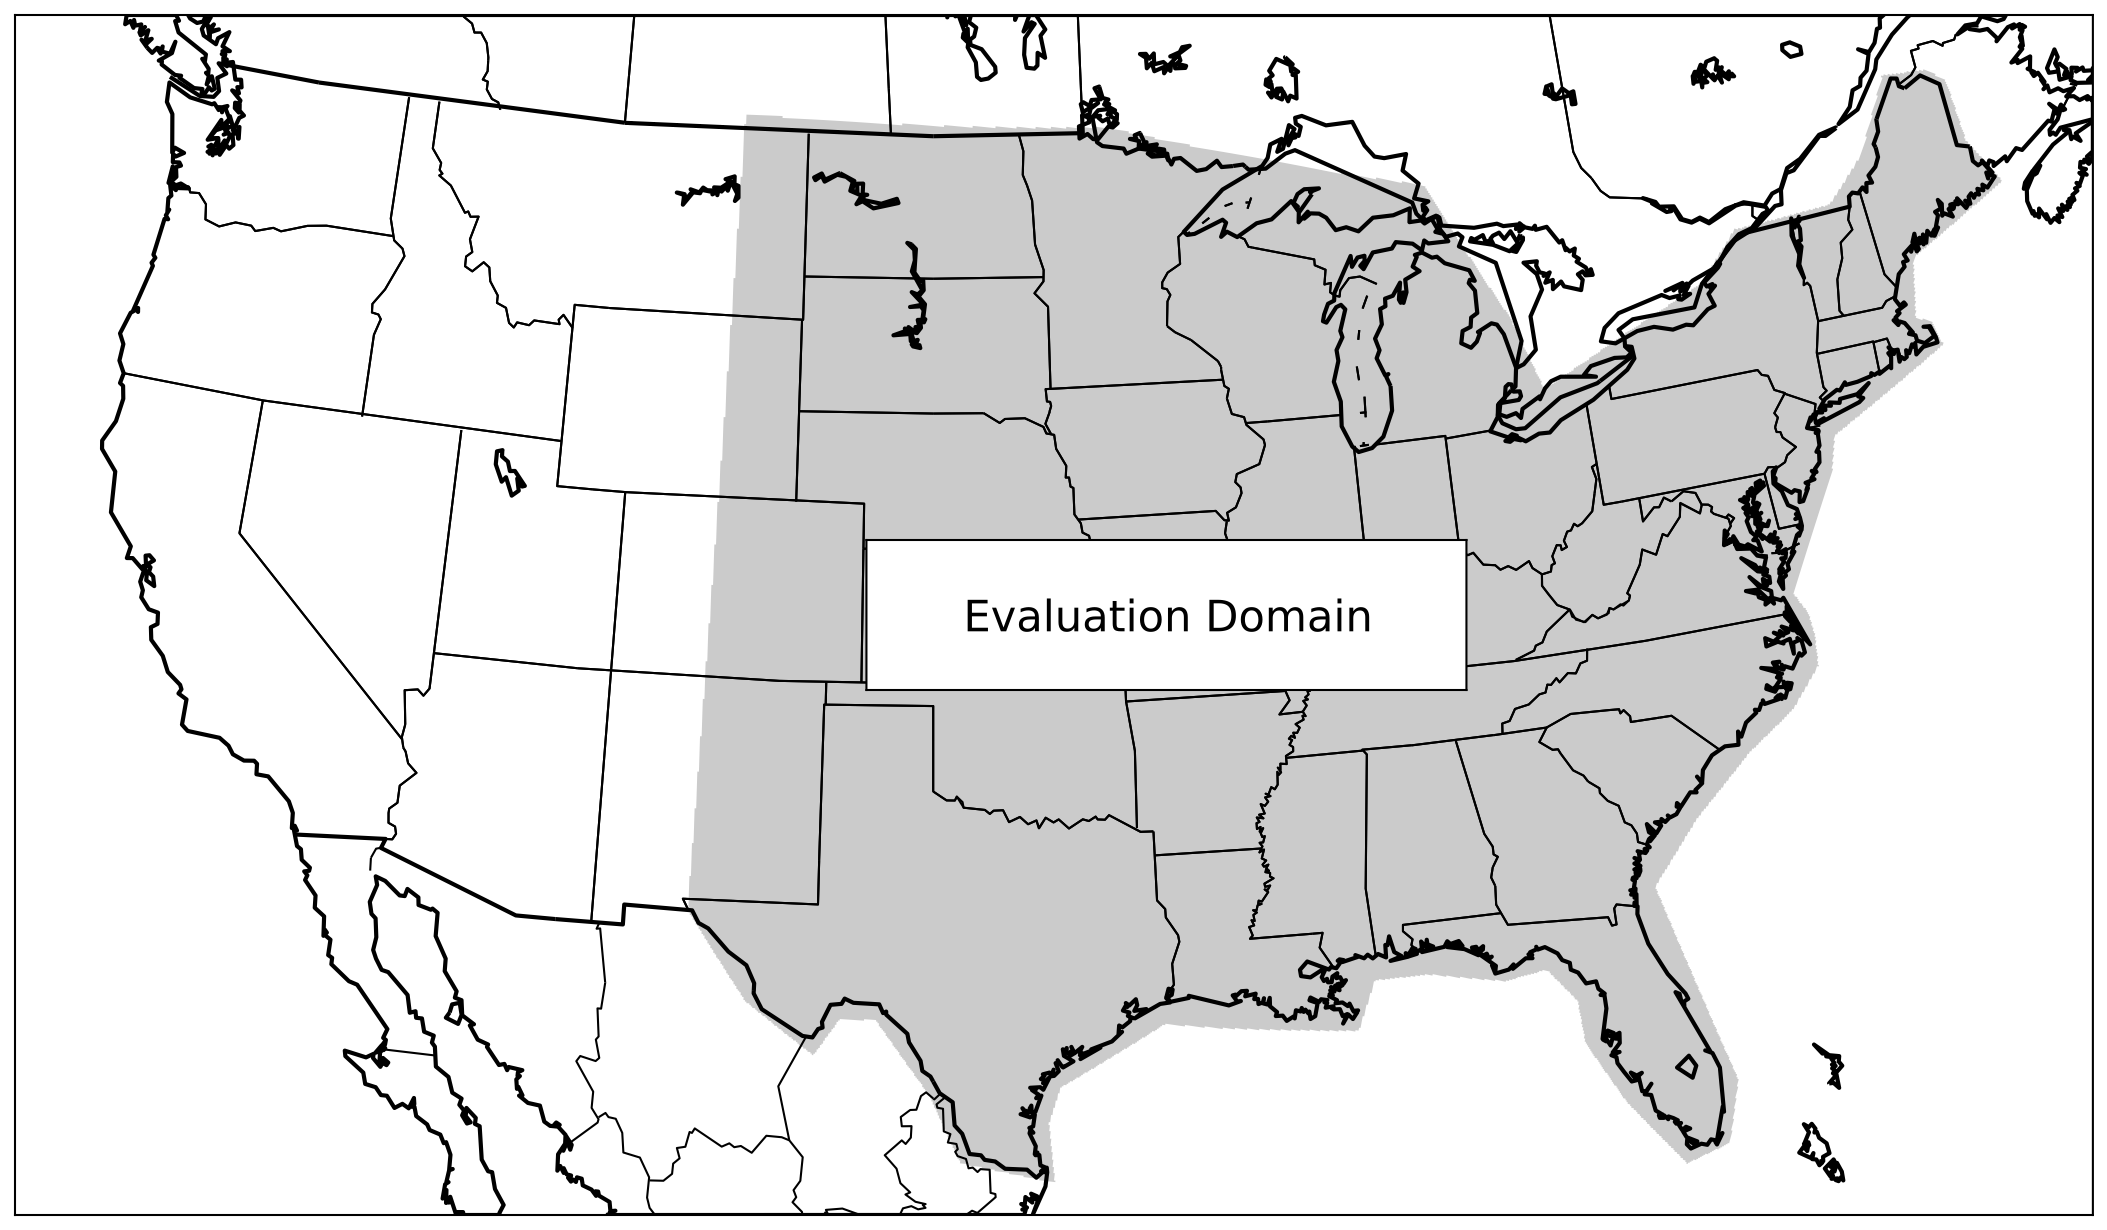
\includegraphics[width=\textwidth, height=\textheight, keepaspectratio]{%
    ./deterministic/figs/domain}\\
    \caption{The subset of the Stage IV grid used in the analysis.}
    \label{domain}
\end{figure}


\clearpage
\begin{figure}[cc]
    \centering
    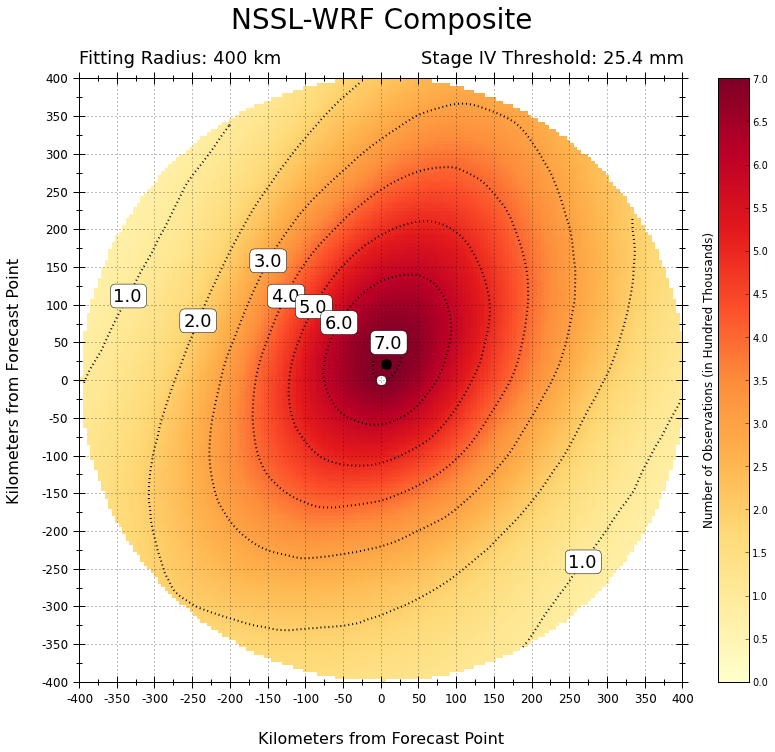
\includegraphics[width=\textwidth, height=\textheight, keepaspectratio]{%
    ./deterministic/figs/single_member_composite_400km_25mm}\\
    \caption{The two-dimensional frequency distribution of stage IV observations greater than or equal to \mbox{25.4 mm} relative to NSSL-WRF forecasts of similar events for the training dataset (1 Apr 2007 -- 31 Mar 2010).
    The representative NSSL-WRF forecast grid point is marked by a white dot in the middle of the domain and the stage IV observation frequency is color filled.
    To illustrate the displacement between forecasts and observations, the centroid of the observations is denoted by the black dot.
    Contour labels are given in hundred-thousands.}
    \label{single_25comp}
\end{figure}


\clearpage
\begin{figure}[cc]
    \centering
    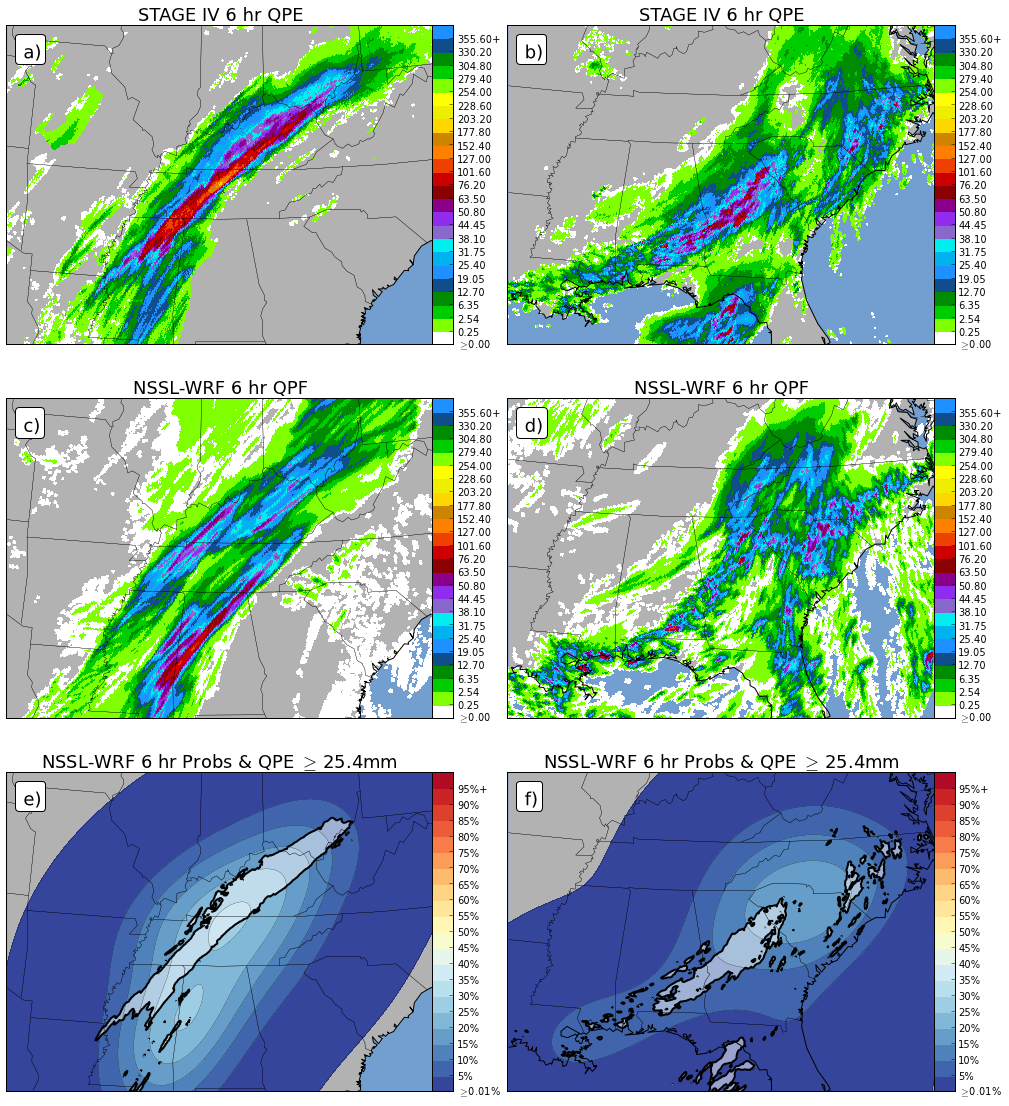
\includegraphics[width=\textwidth, height=\textheight, keepaspectratio]{%
    ./deterministic/figs/single_member_example1_400km_25mm}\\
    \caption{Example forecasts and observations from two separate days and differing forecast lengths.
    The column on the left depicts forecasts and observations for the 6-hrs ending 02 May 2010 at 18 UTC (12-18 hr forecast) whereas the column on the right depicts forecasts and observations for the 6-hrs ending 27 September 2010 at 00 UTC (18-24 hr forecast).
    Panels (a) and (b) denote the Stage IV 6-hr quantitative precipitation estimates (QPE), panels (c) and (d) denote the 6-hr NSSL-WRF 6-hr quantitative precipitation forecasts (QPF), and panels (e) and (f) depict the Stage IV QPE greater than 25.4 mm contoured on top of the NSSL-WRF probability of exceeding 25.4 mm in 6-hrs. The minimum shaded probability is 0.0001 (0.01\%).}
    \label{single_1_400km_25mm}
\end{figure}


\clearpage
\begin{figure}[cc]
    \centering
    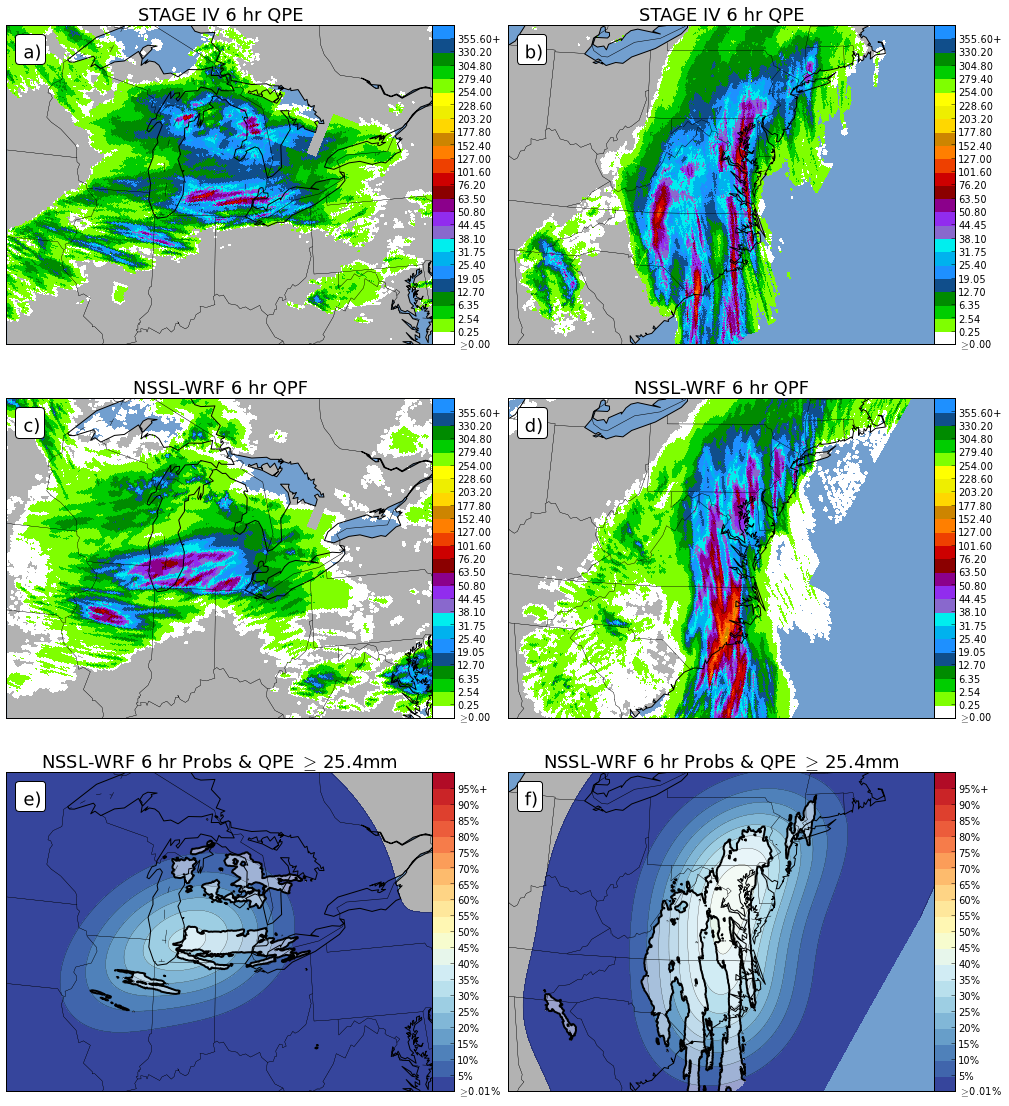
\includegraphics[width=\textwidth, height=\textheight, keepaspectratio]{%
    ./deterministic/figs/single_member_example2_400km_25mm}\\
    \caption{Same layout as in \mbox{Figure \ref{single_1_400km_25mm}} except the left column depicts the forecast and observations for the 6-hrs ending 06 June 2010 at 06 UTC (24-30 hr forecast) and the right column depicts the 6-hrs ending 30 September 2010 at 12 UTC (30-36 hr forecast).}
    \label{single_2_400km_25mm}
\end{figure}


\clearpage
\begin{figure}[cc]
    \centering
    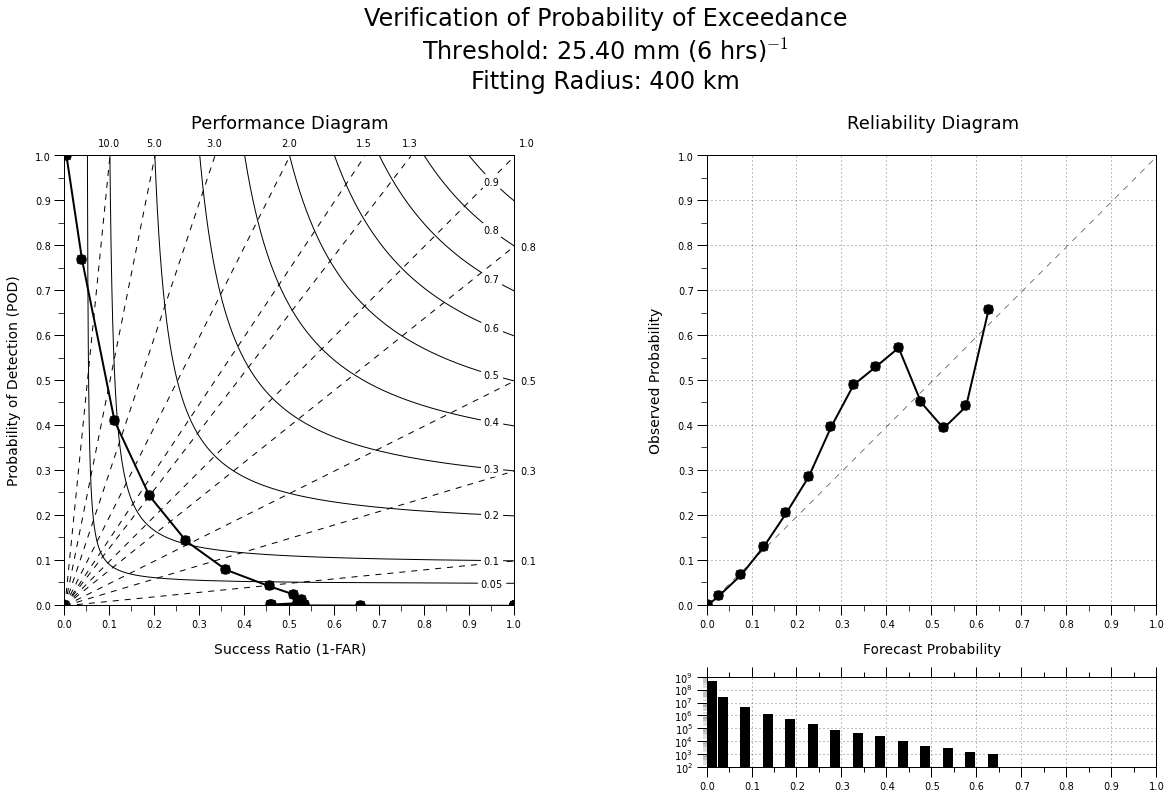
\includegraphics[width=\textwidth, height=\textheight, keepaspectratio]{%
    ./deterministic/figs/single_member_verif_400km_25mm}\\
    \caption{Performance Diagram (a) and reliability diagram with corresponding forecast counts (b), both computed over the 01 April 2010 to 31 March 2011 time period.
    The line of perfect reliability (diagonal; dashed) is also plotted on the reliability diagram.
    The forecast counts associated with the reliability diagram are plotted on a log-scale below the reliability diagram (c).}
    \label{single_verif_400km_25mm}
\end{figure}


\clearpage
\begin{figure}[cc]
    \centering
    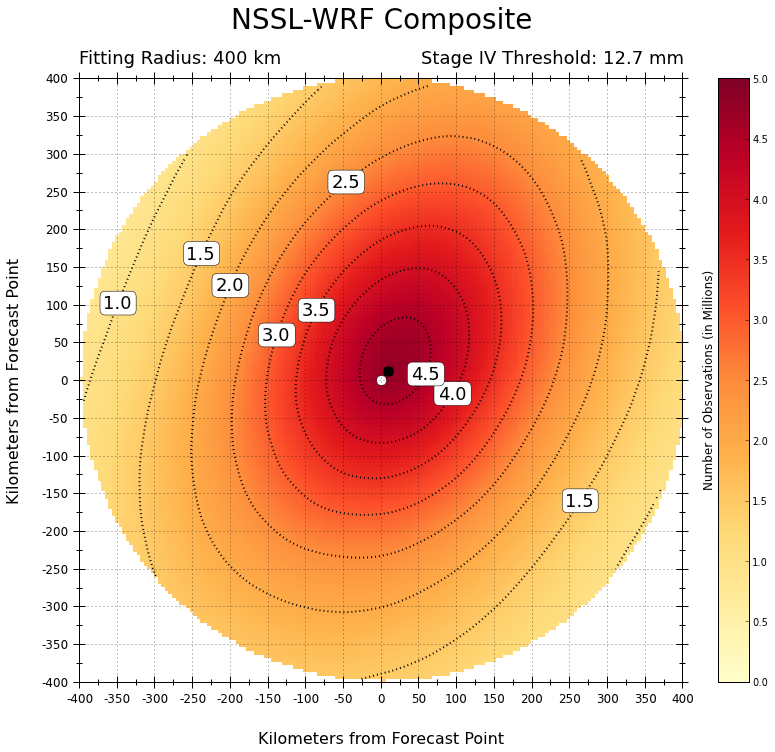
\includegraphics[width=\textwidth, height=\textheight, keepaspectratio]{%
    ./deterministic/figs/single_member_composite_400km_12mm}\\
    \caption{Same as in Figure \ref{single_25comp} except for the \mbox{12.7 mm} threshold and contour labels in millions.}

    \label{single_12comp}
\end{figure}


\clearpage
\begin{figure}[cc]
    \centering
    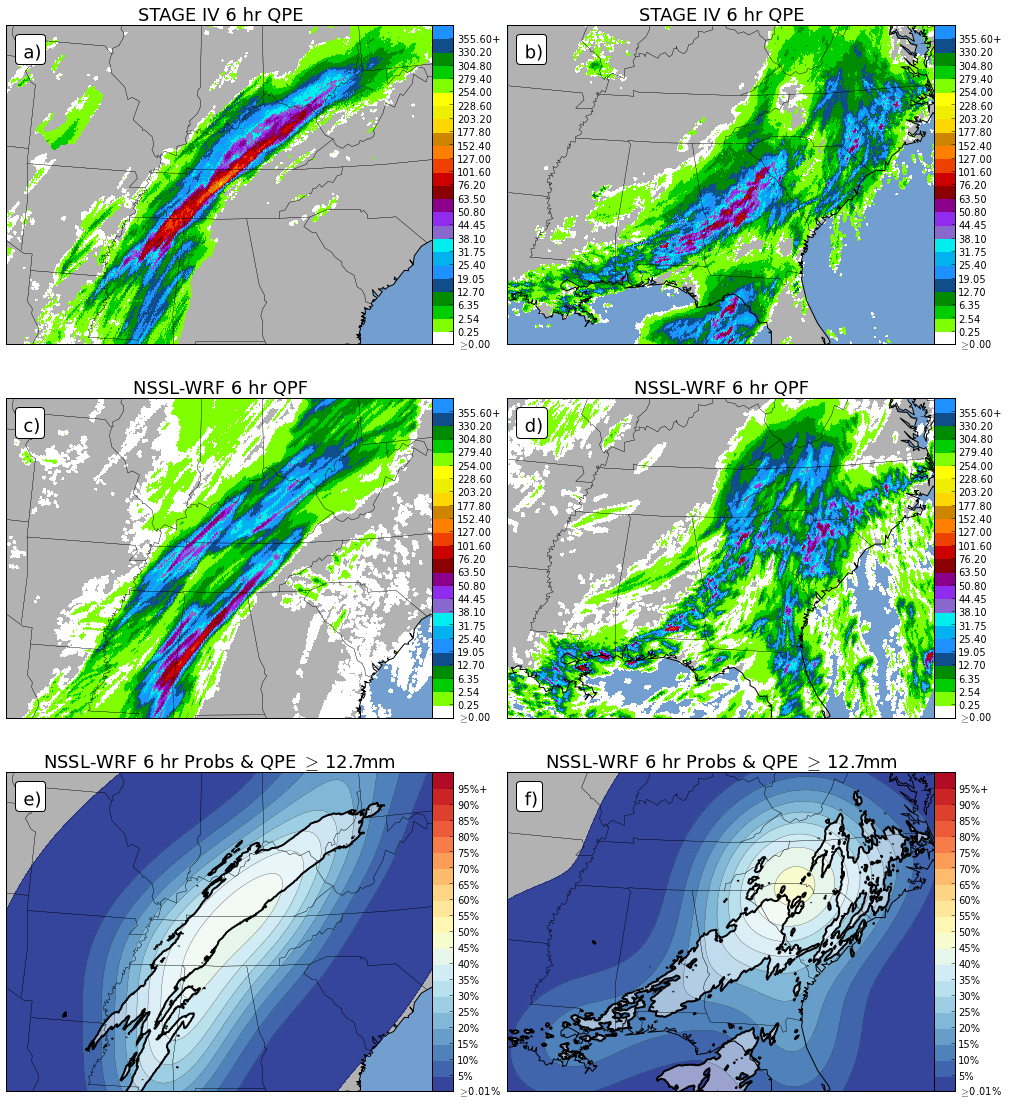
\includegraphics[width=\textwidth, height=\textheight, keepaspectratio]{%
    ./deterministic/figs/single_member_example1_400km_12mm}\\
    \caption{The same as in \mbox{Figure \ref{single_1_400km_25mm}} except using the \mbox{12.7 mm} threshold.}
    \label{single_1_400km_12mm}
\end{figure}


\clearpage
\begin{figure}[cc]
    \centering
    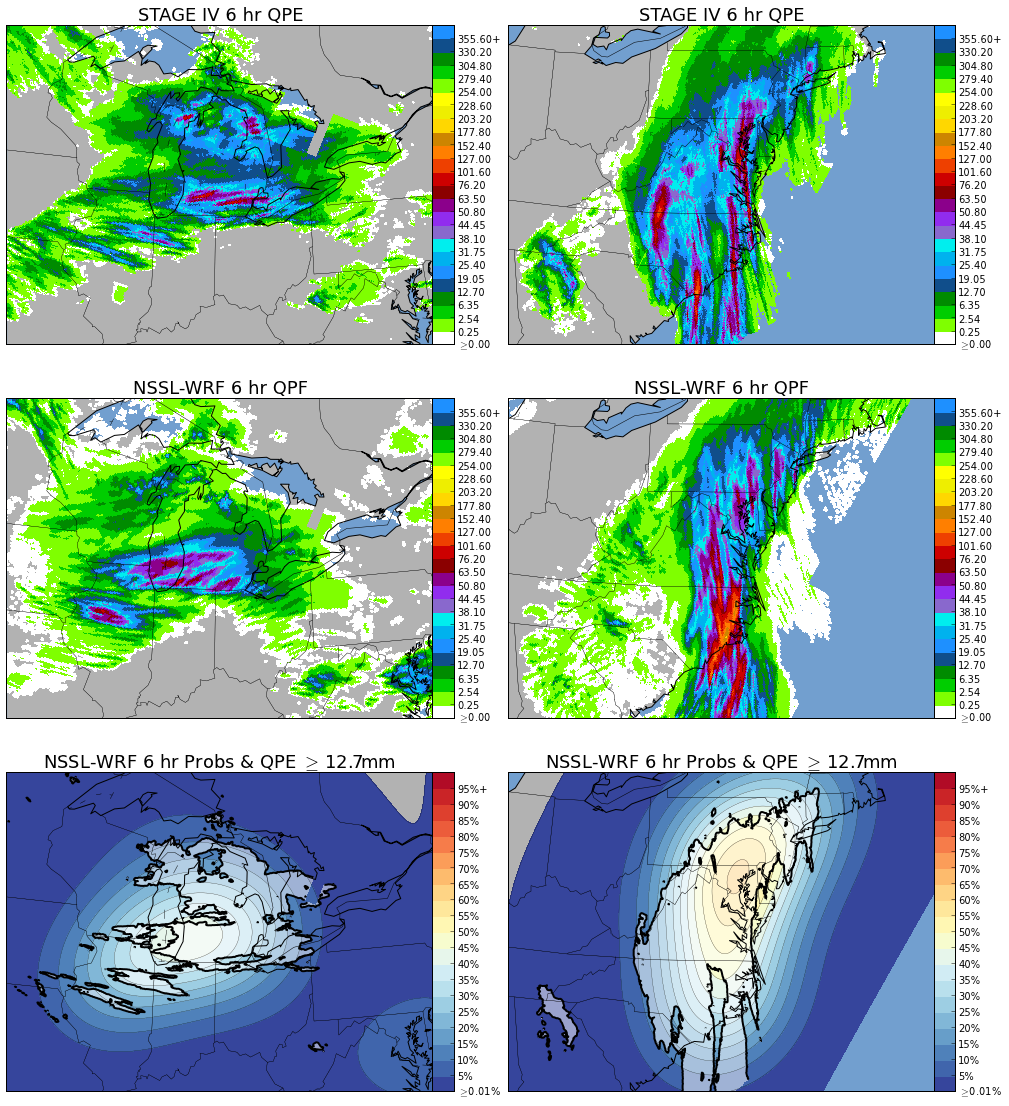
\includegraphics[width=\textwidth, height=\textheight, keepaspectratio]{%
    ./deterministic/figs/single_member_example2_400km_12mm}\\
    \caption{The same as in \mbox{Figure \ref{single_2_400km_25mm}} except using the \mbox{12.7 mm} threshold.}
    \label{single_2_400km_12mm}
\end{figure}


\clearpage
\begin{figure}[cc]
    \centering
    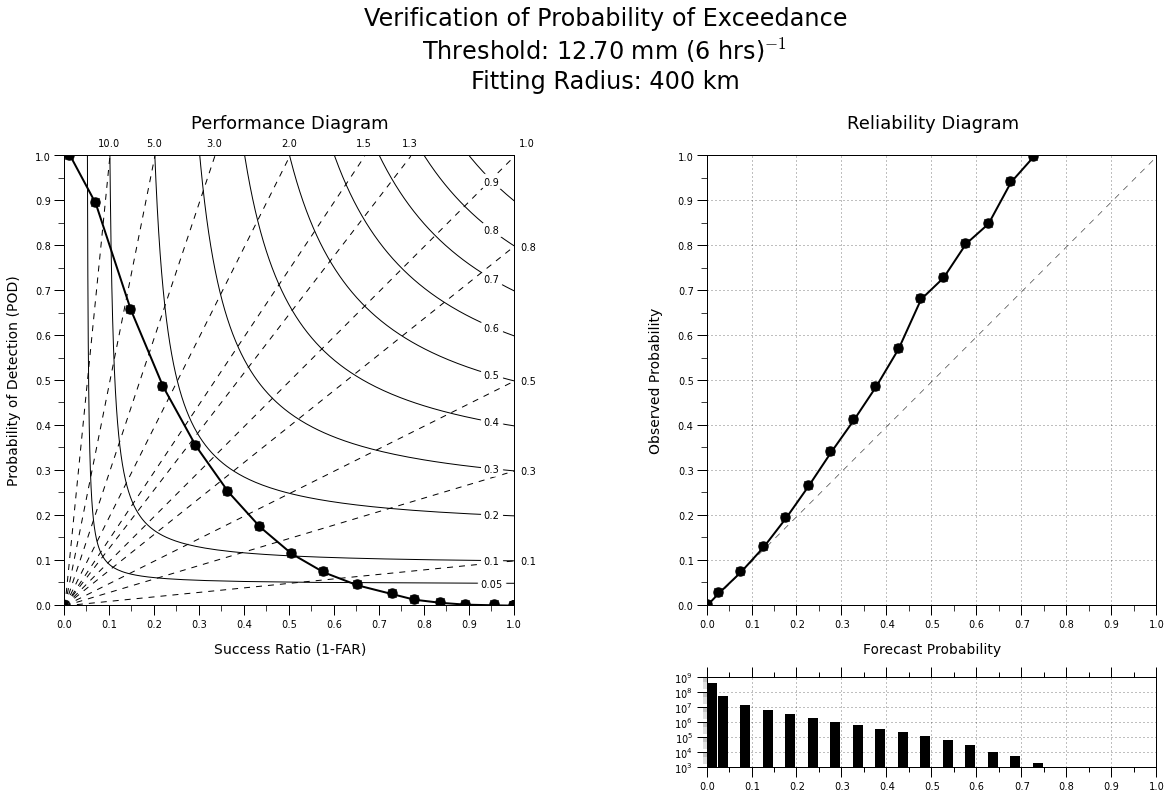
\includegraphics[width=\textwidth, height=\textheight, keepaspectratio]{%
    ./deterministic/figs/single_member_verif_400km_12mm}\\
    \caption{The same as in \mbox{Figure \ref{single_verif_400km_25mm}} except using the \mbox{12.7 mm} threshold.}
    \label{single_verif_400km_12mm}
\end{figure}
